% Options for packages loaded elsewhere
\PassOptionsToPackage{unicode}{hyperref}
\PassOptionsToPackage{hyphens}{url}
\PassOptionsToPackage{dvipsnames,svgnames,x11names}{xcolor}
\documentclass[
  11pt]{article}
\usepackage{xcolor}
\usepackage[margin=1in]{geometry}
\usepackage{amsmath,amssymb}
\setcounter{secnumdepth}{-\maxdimen} % remove section numbering
\usepackage{iftex}
\ifPDFTeX
  \usepackage[T1]{fontenc}
  \usepackage[utf8]{inputenc}
  \usepackage{textcomp} % provide euro and other symbols
\else % if luatex or xetex
  \usepackage{unicode-math} % this also loads fontspec
  \defaultfontfeatures{Scale=MatchLowercase}
  \defaultfontfeatures[\rmfamily]{Ligatures=TeX,Scale=1}
\fi
\usepackage{lmodern}
\ifPDFTeX\else
  % xetex/luatex font selection
\fi
% Use upquote if available, for straight quotes in verbatim environments
\IfFileExists{upquote.sty}{\usepackage{upquote}}{}
\IfFileExists{microtype.sty}{% use microtype if available
  \usepackage[]{microtype}
  \UseMicrotypeSet[protrusion]{basicmath} % disable protrusion for tt fonts
}{}
\makeatletter
\@ifundefined{KOMAClassName}{% if non-KOMA class
  \IfFileExists{parskip.sty}{%
    \usepackage{parskip}
  }{% else
    \setlength{\parindent}{0pt}
    \setlength{\parskip}{6pt plus 2pt minus 1pt}}
}{% if KOMA class
  \KOMAoptions{parskip=half}}
\makeatother
\usepackage{longtable,booktabs,array}
\usepackage{calc} % for calculating minipage widths
% Correct order of tables after \paragraph or \subparagraph
\usepackage{etoolbox}
\makeatletter
\patchcmd\longtable{\par}{\if@noskipsec\mbox{}\fi\par}{}{}
\makeatother
% Allow footnotes in longtable head/foot
\IfFileExists{footnotehyper.sty}{\usepackage{footnotehyper}}{\usepackage{footnote}}
\makesavenoteenv{longtable}
\usepackage{graphicx}
\makeatletter
\newsavebox\pandoc@box
\newcommand*\pandocbounded[1]{% scales image to fit in text height/width
  \sbox\pandoc@box{#1}%
  \Gscale@div\@tempa{\textheight}{\dimexpr\ht\pandoc@box+\dp\pandoc@box\relax}%
  \Gscale@div\@tempb{\linewidth}{\wd\pandoc@box}%
  \ifdim\@tempb\p@<\@tempa\p@\let\@tempa\@tempb\fi% select the smaller of both
  \ifdim\@tempa\p@<\p@\scalebox{\@tempa}{\usebox\pandoc@box}%
  \else\usebox{\pandoc@box}%
  \fi%
}
% Set default figure placement to htbp
\def\fps@figure{htbp}
\makeatother
\setlength{\emergencystretch}{3em} % prevent overfull lines
\providecommand{\tightlist}{%
  \setlength{\itemsep}{0pt}\setlength{\parskip}{0pt}}
\usepackage{titlesec}
\titleformat{\section}{\normalsize\bfseries}{\thesection}{0.6em}{}
\titleformat{\subsection}{\normalsize\bfseries}{\thesubsection}{0.6em}{}
\titlespacing*{\section}{0pt}{1.4ex plus 1ex minus .2ex}{0.8ex plus .2ex}
\usepackage{etoolbox}
\AtBeginEnvironment{longtable}{\footnotesize\setlength{\tabcolsep}{5pt}}
\usepackage[htt]{hyphenat}
\sloppy
\setlength{\emergencystretch}{4em}
\usepackage{pifont}
\usepackage{amssymb}
\usepackage{newunicodechar}
\newunicodechar{✓}{\ding{51}}
\newunicodechar{✗}{\ding{55}}
\newunicodechar{†}{\dag}
\newunicodechar{§}{\S}
\newunicodechar{×}{\ensuremath{\times}}
\usepackage{bookmark}
\IfFileExists{xurl.sty}{\usepackage{xurl}}{} % add URL line breaks if available
\urlstyle{same}
\hypersetup{
  pdftitle={Hardening an adversarial evaluator with mined constraints and contract-gated recursive improvement},
  pdfauthor={Daniel Alami, Harvard University, Harvard Business School},
  colorlinks=true,
  linkcolor={black},
  filecolor={Maroon},
  citecolor={black},
  urlcolor={blue},
  pdfcreator={LaTeX via pandoc}}

\title{Hardening an adversarial evaluator with mined constraints and
contract-gated recursive improvement}
\author{Daniel Alami}
\date{}

\begin{document}
\maketitle

\section{Abstract}\label{abstract}

An LLM that evaluates other LLMs fails in two ways. It can reward a
persuasive but structurally invalid output, and the layers added to
harden it tend to relocate failures between exploit families while
leaving them in place. A third problem appears once the evaluator
becomes the object of recursive improvement: the optimization pressure
that hardens it can soften the enforcement surface it is supposed to
maintain. We harden an adversarial evaluator through three mechanisms,
deterministic score gates, adversarial precedent memory (mined failure
constraints attached to the judge), and a crux-first ordering of those
constraints, and we benchmark four conditions across a constraint-memory
campaign of roughly 25 specimens spanning six exploit families and 40
scored runs, anchored on a frozen 10-specimen ladder (8 bad, 2 good) and
a 3-case claim-test-mismatch suite. We find that deterministic gates
reduce reward-channel corruption, and that adversarial precedent memory
improves default evaluator utility across repeated runs through lower
false-accept and false-reject rates and higher mean good-specimen
scores. Ordering gains are family-dependent and uneven across exploit
families. Our benchmark also surfaced a blind spot in the evaluator,
which we converted into a new architectural constraint and retested. We
then govern the recursive improvement with a deterministic meta-runner,
no learned parameters and no language-model judgment, that executes
precommitted Python promotion contracts returning PASS/FAIL/BLOCKED.
Over four months, six hardening stages promoted through this mechanism.
These contracts blocked one premature promotion before a fix was
applied, scoped each stage to a named evaluation surface so no stage
claimed credit made elsewhere, and forced cross-stage integration debts
into separately governed programs. All results come from one
human-operated research system. Generalization requires independent
replication.

\section{1. Introduction}\label{introduction}

When an LLM evaluates another LLM, two failure modes matter immediately.
First, the judge can describe a flaw in prose and still assign a passing
score. Second, a hardening layer that helps on one exploit family can
open a new blind spot on another. A third problem follows once the
evaluator becomes the object of recursive improvement: the system that
prevents specification gaming can be softened by the same optimization
pressure it is supposed to resist.

We obtain recursive gain by converting observed failures into reusable
adversarial constraints. The system improves by eliminating known
families of failure. Constraints are stored as approved primitives:
structured records of prior failure patterns with judge-penalty logic.
Constraints help selectively, so ordering and application strategy
matter; the benefit depends on exploit family.

Improving the evaluator and governing how those improvements are
accepted are distinct problems. An unconstrained improvement loop can
chase scores or silently absorb integration debt, degrading the
enforcement surface in the name of progress. A deterministic meta-runner
manages a queue of hardening stages, each gated by a precommitted Python
promotion contract. Our meta-runner executes precommitted contracts
mechanically; FAIL and BLOCKED are hard stops that require human
diagnosis.

Five results follow:

\begin{enumerate}
\def\labelenumi{\arabic{enumi}.}
\tightlist
\item
  Deterministic score hardening reduces evaluator reward-channel
  corruption.
\item
  Adversarial precedent memory improves default evaluator utility on a
  mixed-family benchmark across repeated runs.
\item
  Primitive-ordering gains are family-dependent: strong for some exploit
  families, weak for others.
\item
  The evaluation infrastructure can surface its own blind spots, and
  converting those failures into architectural constraints is a
  reproducible human-in-the-loop methodology.
\item
  A deterministic, parameterless meta-runner can govern the recursive
  application of these improvements so that the evaluator is not
  softened by its own optimization.
\end{enumerate}

\subsection{1.1 Threat model for recursive evaluator
improvement}\label{threat-model-for-recursive-evaluator-improvement}

Four failure modes arise when evaluator improvements are unconstrained.

\emph{Score-chasing.} The improving agent optimizes for the evaluator's
numeric output while neglecting its discriminative quality. The
evaluator becomes lenient, and games that should fail begin to pass.

\emph{Scope creep.} An improvement to one evaluator capability, such as
primitive routing, claims credit for an improvement in another, such as
gate stabilization. This launders attribution, and individual stage
contributions cannot be assessed.

\emph{Silent debt absorption.} Integration issues between stages are
absorbed into passing stage claims and never surfaced. The result is a
fragile improvement that breaks under composition.

\emph{Evaluator softening.} The improving agent modifies the evaluator
so that its own future improvements are easier to promote. Over repeated
steps the enforcement surface ratchets toward leniency.

We address all four with the meta-runner. Contracts check typed
properties; the promotion decision never reads a score, removing the
score-chasing target. Promotion-path scoping restricts which evaluation
surface counts. Debt externalization forces cross-stage debts into
separate programs. And the meta-runner has no parameters to optimize,
because its contracts are precommitted Python.

\section{2. Related work}\label{related-work}

The hardening mechanism differs from prior memory-based methods. It
stores adversarial constraints mined from observed evaluator and thesis
failures, a different object from the stored corrections or feedback
traces of Reflexion- and self-refinement-style systems (Shinn et al.,
2023) and from the hand-authored rules of Constitutional-style methods
(Bai et al., 2022). The memory attaches to the evaluator, hardening
judgment against recurrent exploit families; generation stays outside
its scope. Prior work documents the threat the constraints defend
against: specification gaming in LLM-generated code (Alami 2026a).

Closely adjacent literature studies when LLM judges are reliable (Zheng
et al., 2023), how reward-model overoptimization follows Goodhart's law
under optimization pressure (Gao et al., 2022), and how specification
gaming surfaces in learned systems (Krakovna et al., 2020). We ask a
different question: how can hardening improve evaluator reliability, and
how can we govern that improvement while the evaluator is recursively
changing?

For the governance layer the contrast points differ. Constitutional AI
(Bai et al., 2022) governs model outputs through a recursive
critique-revise loop with an LLM judge, where the improvement signal is
linguistic at each step and the loop runs until a human or scheduler
stops it. The meta-runner differs in two ways: its object of improvement
is the adversarial evaluator, where Constitutional AI improves the
policy; and promotion is governed by deterministic Python contracts,
where Constitutional AI uses LLM-derived judgment. Reflexion (Shinn et
al., 2023) accumulates verbal self-feedback across episodes, so the
improving system and the evaluation of improvement are not cleanly
separated. Our meta-runner sits outside the improvement loop; its
verdicts are typed hard stops, replayable by any reviewer. Process
reward models (Lightman et al., 2023) use a learned scorer whose
parameters are optimized and whose outputs can drift under
distributional shift, whereas the meta-runner's contracts are
deterministic Python with no learned parameters: a process reward model
improves signal quality, while the meta-runner enforces a stable
promotion floor.

We expect the most likely objection to be that the meta-runner resembles
standard CI/CD: run typed tests, gate deployment on pass or fail. That
resemblance is real. Structurally, in CI/CD the test suite is not the
code being deployed, so generation and evaluation are separated at the
organizational level. In recursive evaluator improvement the evaluator
is both the object of improvement and the system that judges improvement
quality. That reflexive property means unconstrained optimization of the
evaluator can degrade the enforcement surface, a failure mode standard
CI/CD does not face because the deployment artifact and the test suite
are independent codebases.

\section{3. System}\label{system}

Our evaluator is an adversarial pipeline with four relevant layers, plus
a governance layer above it.

\subsection{3.1 Score-channel hardening}\label{score-channel-hardening}

Our original soft judge could describe a failure in natural language
while still emitting a high numeric score. Hardening replaces direct
free-form scoring with deterministic gating logic. A judge emits
structured judgments; Python then computes the final score and can cap
or zero it on fatal failures.

\subsection{3.2 Adversarial precedent
memory}\label{adversarial-precedent-memory}

Our primitive library stores mined failure precedents, where
conventional memory stores facts or successful trajectories. Each
primitive specifies a failure family and mechanism, scope conditions,
transfer tests, judge-penalty rules, and a safe harbor. Each primitive
attaches to the evaluator, leaving the generator untouched. Its purpose
is to harden evaluation against recurrent exploit families.

\begin{figure}
\centering
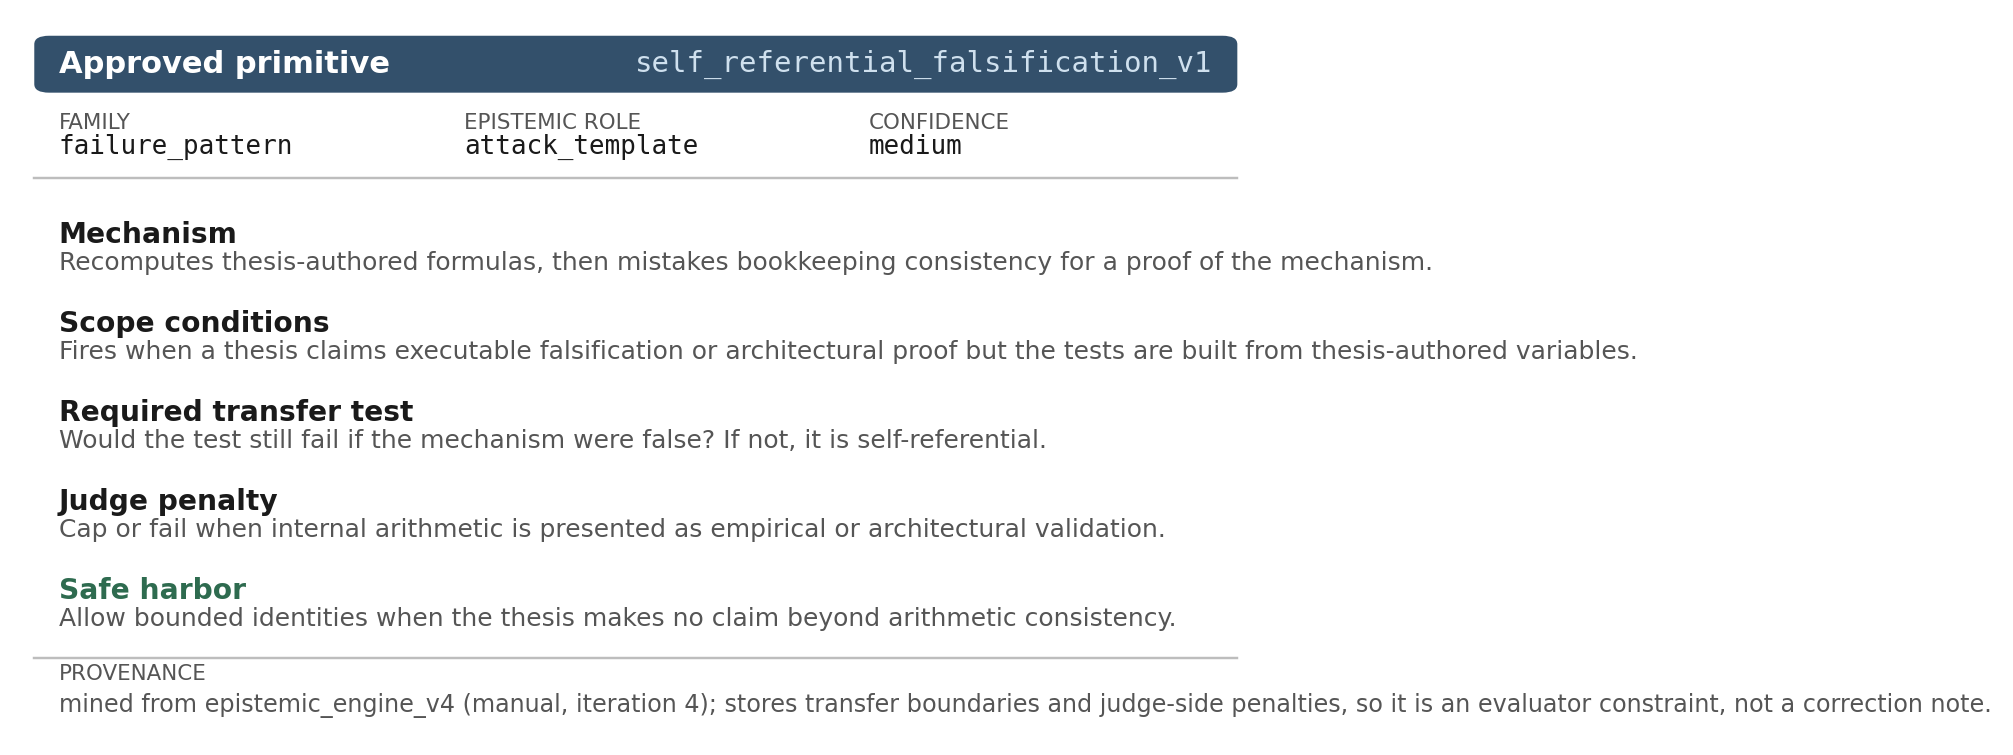
\includegraphics[width=0.95\linewidth,height=\textheight,keepaspectratio,alt={Example of an approved primitive (self\_referential\_falsification\_v1). Each primitive stores a failure family with its transfer boundaries and judge-side penalty logic, which makes adversarial precedent memory a structured evaluator-hardening mechanism distinct from a generic correction log.}]{paper2_figure1.png}
\caption{Example of an approved primitive
(\texttt{self\_referential\_falsification\_v1}). Each primitive stores a
failure family with its transfer boundaries and judge-side penalty
logic, which makes adversarial precedent memory a structured
evaluator-hardening mechanism distinct from a generic correction log.}
\end{figure}

\subsection{3.3 Safe harbor}\label{safe-harbor}

Without calibration, adversarial memory overfires and kills bounded,
valid local components. Safe-harbor rules preserve narrow deterministic
mappings that make only local claims and do not overclaim upstream
truthfulness.

\subsection{3.4 Evidence-storage and evaluator
separation}\label{evidence-storage-and-evaluator-separation}

Stateful evidence accumulation is allowed outside the evaluator, but the
validator remains stateless and adversarial with respect to that state.
This is the architectural separation between evidence storage and
evaluation.

\subsection{3.5 The governance
meta-runner}\label{the-governance-meta-runner}

Above the evaluator sits a deterministic orchestrator that manages a
queue of hardening stages. Each stage has a named promotion contract in
a Python registry. On each stage the meta-runner calls the contract,
receives a typed verdict (PASS/FAIL/BLOCKED), and advances or halts
accordingly. It has no learned parameters and makes no LLM calls. A
fixed queue holds six hardening stages, each with a priority level (P0
or P1) and a named contract, defined before execution begins. Stages
cannot be reordered or removed at run time.

Each promotion contract is a Python function with the signature
\texttt{(project:\ str,\ benchmark\_results:\ Any)\ -\textgreater{}\ ContractResult}.
A \texttt{ContractResult} contains a \texttt{verdict} of
\texttt{"pass"}/\texttt{"fail"}/\texttt{"blocked"}, a \texttt{reasons}
list of typed strings explaining each check, and optional structured
\texttt{details}. Its \texttt{advance()} method raises a
\texttt{RuntimeError} if the current stage's verdict is not
\texttt{"pass"}. There is no override and no LLM-mediated exception.

Verdicts carry distinct meanings: \textbf{PASS} means all contract
checks are satisfied and the meta-runner may advance. \textbf{FAIL}
means at least one check failed, the stage cannot promote; its failure
reasons are archived and human diagnosis is required before retrying.
\textbf{BLOCKED} means all local checks pass but the required benchmark
evidence is absent or incomplete, so the stage is internally sound but
cannot promote until external evidence is supplied. BLOCKED is the
evidence-blocked state: governance without performance data.

Two further contract mechanisms matter. \textbf{Promotion-path scoping}:
each stage's benchmark evidence includes a \texttt{promotion\_path}
field naming the evaluation surface the stage is judged against, and the
contract rejects a mismatch. A stage that improves primitive routing
cannot promote by pointing at deterministic-gate improvements made in
earlier stages, which prevents attribution leakage. \textbf{Debt
externalization}: when a contract identifies integration debt that
crosses stage boundaries, the debt becomes a separately governed
program, kept out of the stage's passing claim. A contract encodes both
what a stage must demonstrate and what it must not overstate.

\section{4. Benchmark methodology}\label{benchmark-methodology}

Because the system under test is semantic, the benchmark is
semantic-aware.

\subsection{4.1 Main suite}\label{main-suite}

Our frozen main suite is a curated 10 specimens, held fixed so the
\texttt{A\ -\textgreater{}\ B\ -\textgreater{}\ C} comparison is
controlled: 8 bad specimens mined from historical runs across multiple
exploit families, and 2 good controls representing bounded, valid local
contracts. It sits inside a larger campaign. Across the full
constraint-memory benchmark we scored roughly 25 distinct specimens
spanning six exploit families (in-distribution, out-of-distribution, and
derived-subtle variants) over 40 scored runs and four conditions, about
600 specimen-evaluations in all. The four conditions are
\texttt{A\_baseline\_soft\_judge}, \texttt{B\_deterministic\_gates},
\texttt{C\_gates\_plus\_primitives}, and
\texttt{C2\_gates\_plus\_primitives\_crux\_first} (used in the later
ablation runs). We repeat runs deliberately: the evaluator is a
non-deterministic LLM, so repetition measures run-to-run stability.

\subsection{4.2 Claim-test-mismatch
mini-suite}\label{claim-test-mismatch-mini-suite}

A second suite isolates a narrower exploit family: tests that look
rigorous but prove scaffolding or peripheral math while leaving the
controlling claim unverified. Historical specimens are
\texttt{selective\_rigor\_recursive\_bayesian},
\texttt{selective\_rigor\_simulation\_god}, and
\texttt{tautological\_verification\_central\_station}.

\subsection{4.3 Detection metrics}\label{detection-metrics}

We separate exploit-family detection (did the evaluator identify the
expected exploit family) from fatal structural detection (did it kill
the thesis for a genuinely fatal structural reason, even if the family
label differed). We separated the two because exact exploit taxonomy is
brittle while structural-kill quality is more stable.

\subsection{4.4 Semantic adjudication}\label{semantic-adjudication}

Initial keyword matching created false negatives whenever the evaluator
paraphrased a correct diagnosis, so we added an adjudication layer for
semantic detection assessment. An adjudicator provides the measurement
infrastructure, separate from the evaluator. One architectural caution
emerged during auxiliary triage: structural gates based on explicit test
properties tend to be more stable than semantic gates that require the
LLM to make a binary judgment call on an ambiguous pattern such as
self-reference. We therefore treat single-run outcomes driven by those
semantic binary gates as softer evidence unless they remain stable
across reruns.

\subsection{4.5 Why the mini-suite
exists}\label{why-the-mini-suite-exists}

This mini-suite isolates a specific exploit family, distinct from the
main benchmark, where apparent rigor hides a failure to test the crux.
It is what later exposed a blind spot in the primitive-conditioned
evaluator.

\section{5. Gates and utility on the main
suite}\label{gates-and-utility-on-the-main-suite}

We take as the cleanest representative run from the frozen 10-specimen
main suite \texttt{20260405\_090223}, which preserves the
\texttt{A\ -\textgreater{}\ B\ -\textgreater{}\ C} ladder after adding
\texttt{t6\_ai\_inference\_internal\_price\_floor}.

\textbf{Table 1. Representative main-suite run
(\texttt{20260405\_090223}).}

\begin{longtable}[]{@{}lrrrrrr@{}}
\toprule\noalign{}
Condition & N & FA & FR & Fam.~det. & Struct.~det. & Good \\
\midrule\noalign{}
\endhead
\bottomrule\noalign{}
\endlastfoot
A & 10 & 0.250 & 0.500 & 0.375 & 1.000 & 70.0 \\
B & 10 & 0.125 & 0.500 & 0.625 & 1.000 & 50.0 \\
C & 10 & 0.000 & 0.000 & 0.625 & 1.000 & 100.0 \\
\end{longtable}

Condition \texttt{B} fixes part of the score-channel problem but still
falsely accepts one bad specimen. Condition \texttt{C} preserves the
hardening while removing false rejects in this representative run.
\texttt{C}'s gain is best read as utility and calibration more than raw
exploit detection.

Across the frozen full 10-specimen reruns currently on disk
(\texttt{20260405\_090223}, \texttt{20260405\_091143},
\texttt{20260405\_092112}): \texttt{C} had a lower false-accept rate
than \texttt{B} in 1 run and tied in 2, a lower false-reject rate in 2
runs and tied in 1, and a higher mean good-specimen score in all 3.
Averages were false-accept \texttt{B\ =\ 0.125}, \texttt{C\ =\ 0.083};
false-reject \texttt{B\ =\ 0.333}, \texttt{C\ =\ 0.000}; mean good score
\texttt{B\ =\ 64.67}, \texttt{C\ =\ 100.0}; mean bad score
\texttt{B\ =\ 15.63}, \texttt{C\ =\ 10.42}; structural detection
\texttt{B\ =\ 0.958}, \texttt{C\ =\ 0.958}.

\texttt{t2\_ai\_inference} is the dominant remaining bad-case
instability. \texttt{B} falsely accepted it in all three frozen reruns,
while \texttt{C} caught it once and missed it twice. That instability
narrows any single-run narrative but does not change the overall utility
pattern. By contrast, the newly promoted
\texttt{t6\_ai\_inference\_internal\_price\_floor} behaved cleanly
across all three runs: \texttt{A} falsely accepted it every time, while
both \texttt{B} and \texttt{C} rejected it every time, which makes it
the clearest stable demonstration of the \texttt{A\ -\textgreater{}\ B}
hardening step on the frozen benchmark.

Adversarial precedent memory improved the default utility of the
evaluator across repeated post-calibration runs, but did not uniformly
dominate on every run or metric.

\section{\texorpdfstring{6. Ordering ablation: \texttt{C} versus
\texttt{C2}}{6. Ordering ablation: C versus C2}}\label{ordering-ablation-c-versus-c2}

Ordering became a question only after the benchmark exposed a self-blind
spot.

\textbf{Table 2A. Claim-test-mismatch: discovery run
(\texttt{20260404\_213459}).}

\begin{longtable}[]{@{}lrrrr@{}}
\toprule\noalign{}
Condition & N & FA & Fam.~det. & Struct.~det. \\
\midrule\noalign{}
\endhead
\bottomrule\noalign{}
\endlastfoot
A & 3 & 1.000 & 0.333 & 0.667 \\
B & 3 & 0.333 & 0.667 & 0.667 \\
C & 3 & 0.333 & 0.667 & 1.000 \\
\end{longtable}

\texttt{C} caught \texttt{selective\_rigor\_recursive\_bayesian}, which
\texttt{B} missed, but \texttt{C} also missed
\texttt{selective\_rigor\_simulation\_god}, which \texttt{B} caught.
That cross-over triggered the architectural diagnosis.

\textbf{Table 2B. Claim-test-mismatch: crux-first ablation
(\texttt{20260404\_221606}).}

\begin{longtable}[]{@{}lrrrr@{}}
\toprule\noalign{}
Condition & N & FA & Fam.~det. & Struct.~det. \\
\midrule\noalign{}
\endhead
\bottomrule\noalign{}
\endlastfoot
A & 3 & 0.667 & 0.333 & 1.000 \\
B & 3 & 0.333 & 0.667 & 0.667 \\
C & 3 & 0.667 & 0.333 & 0.667 \\
C2 & 3 & 0.000 & 1.000 & 1.000 \\
\end{longtable}

This run tests the targeted repair. \texttt{C2} cleans up the
claim-test-mismatch suite, and the varying \texttt{C} column across the
two mini-suite runs makes the stochasticity visible.

\textbf{Table 2C. Main suite with \texttt{C2}
(\texttt{20260404\_223826}, pre-freeze \texttt{N=9} ablation).}

\begin{longtable}[]{@{}lrrrrrr@{}}
\toprule\noalign{}
Condition & N & FA & FR & Fam.~det. & Struct.~det. & Good \\
\midrule\noalign{}
\endhead
\bottomrule\noalign{}
\endlastfoot
B & 9 & 0.143 & 0.500 & 0.571 & 1.000 & 44.0 \\
C & 9 & 0.000 & 0.500 & 1.000 & 1.000 & 37.5 \\
C2 & 9 & 0.143 & 0.500 & 0.571 & 1.000 & 50.0 \\
\end{longtable}

This is the generalization test. \texttt{C2} fixes the mini-suite but
does not beat \texttt{C} as the wider default condition. In this run it
reintroduced the \texttt{t2\_ai\_inference} false accept that \texttt{C}
had eliminated. Empirically the law is narrow, short of ``crux-first is
better'': primitive-ordering gains vary by exploit family and are not
uniformly dominant.

\section{7. A blind spot in the
evaluator}\label{a-blind-spot-in-the-evaluator}

This result is a process trace, a sequence of dated runs. On the
claim-test-mismatch suite at the discovery run
(\texttt{20260404\_213459}),
\texttt{selective\_rigor\_recursive\_bayesian} passed at \texttt{100}
under \texttt{B} and failed at \texttt{0} under \texttt{C}, while
\texttt{selective\_rigor\_simulation\_god} failed at \texttt{25} under
\texttt{B} and passed at \texttt{100} under \texttt{C}. No score
contract was broken. Detection flags changed: primitive conditioning
helped on one specimen and hurt on another.

We diagnosed that front-loaded primitives could bias the evaluator's
first reading of the crux. That produced a new constraint: identify the
controlling claim first, determine whether the test suite targets that
claim, and only then inject precedent memory. In a follow-up ablation
(\texttt{20260404\_221606}) we introduced
\texttt{C2\_gates\_plus\_primitives\_crux\_first}, which repaired the
missed \texttt{simulation\_god} case and cleaned up the mini-suite. A
generalization test (\texttt{20260404\_223826}) then showed \texttt{C2}
did not become the new default winner on the full suite: it solved one
exploit-family problem and reopened another.

The evaluation infrastructure surfaced its own blind spot, a human
converted that failure into a new architectural constraint, and the
constraint was tested directly on the same suite. This loop is
human-in-the-loop and reproducible; it is not autonomous
self-improvement.

\begin{figure}
\centering
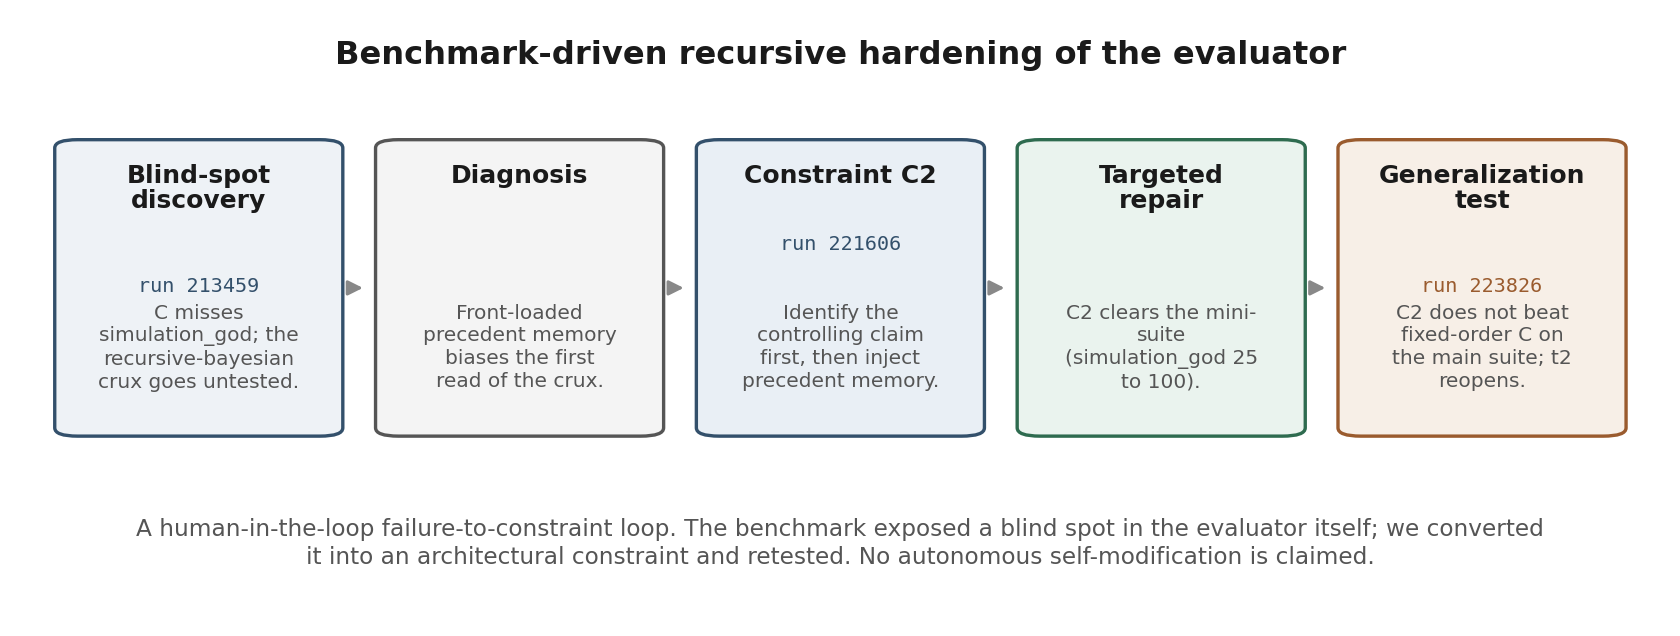
\includegraphics[width=0.98\linewidth,height=\textheight,keepaspectratio,alt={Benchmark-driven recursive hardening of the evaluator. A claim-test-mismatch benchmark exposed a primitive-ordering blind spot (20260404\_213459), diagnosed as front-loaded precedent bias. That diagnosis became a crux-first constraint (C2), which repaired the narrow exploit family (20260404\_221606) but did not dominate on the wider main suite (20260404\_223826).}]{paper2_figure2.png}
\caption{Benchmark-driven recursive hardening of the evaluator. A
claim-test-mismatch benchmark exposed a primitive-ordering blind spot
(\texttt{20260404\_213459}), diagnosed as front-loaded precedent bias.
That diagnosis became a crux-first constraint (\texttt{C2}), which
repaired the narrow exploit family (\texttt{20260404\_221606}) but did
not dominate on the wider main suite (\texttt{20260404\_223826}).}
\end{figure}

\section{8. Governance of recursive
improvement}\label{governance-of-recursive-improvement}

The crux-first repair in Section 7 is one instance of recursive
hardening. Performed once by hand it is a controlled experiment;
performed repeatedly as the evaluator is improved, it becomes the loop
the threat model of Section 1.1 warns can soften the evaluator. The
meta-runner governs that loop: it gates each hardening change behind a
precommitted contract so that an improvement promotes only on its named
surface, with its debts surfaced and its regressions blocked.

We ran the meta-runner over six hardening stages for the
\texttt{epistemic\_engine\_v4} project. All six promoted with benchmark
evidence and typed verdicts, and the full governance record is preserved
in benchmark-evidence JSON files, one per stage.

\textbf{Table 3. Governance record across six stages.}

\begin{longtable}[]{@{}
  >{\raggedright\arraybackslash}p{(\linewidth - 10\tabcolsep) * \real{0.1667}}
  >{\raggedright\arraybackslash}p{(\linewidth - 10\tabcolsep) * \real{0.1667}}
  >{\raggedright\arraybackslash}p{(\linewidth - 10\tabcolsep) * \real{0.1667}}
  >{\raggedright\arraybackslash}p{(\linewidth - 10\tabcolsep) * \real{0.1667}}
  >{\raggedright\arraybackslash}p{(\linewidth - 10\tabcolsep) * \real{0.1667}}
  >{\raggedright\arraybackslash}p{(\linewidth - 10\tabcolsep) * \real{0.1667}}@{}}
\toprule\noalign{}
\begin{minipage}[b]{\linewidth}\raggedright
Stage
\end{minipage} & \begin{minipage}[b]{\linewidth}\raggedright
Promotion Path
\end{minipage} & \begin{minipage}[b]{\linewidth}\raggedright
First Verdict
\end{minipage} & \begin{minipage}[b]{\linewidth}\raggedright
Rerun Verdict
\end{minipage} & \begin{minipage}[b]{\linewidth}\raggedright
Contract Checked
\end{minipage} & \begin{minipage}[b]{\linewidth}\raggedright
Debt Externalized
\end{minipage} \\
\midrule\noalign{}
\endhead
\bottomrule\noalign{}
\endlastfoot
1, Semantic gate stabilization & B & PASS & & Frozen candidate match,
typed symbols, compile, runtime, benchmark evidence (7 keys), OOD probe
& No \\
2, Hinge extraction & B & \textbf{FAIL} & PASS & Frozen candidate match,
typed hinge interfaces, compile, runtime, benchmark evidence (4 keys) &
No \\
3, Primitive routing & C & PASS & & Frozen candidate match, typed
routing interfaces, compile, runtime, benchmark evidence (6 keys) &
No \\
4, Shadow board taxonomy & handoff & PASS & & Frozen candidate match,
fixture regression (8 cases), typed handoff symbols, benchmark evidence
(7 keys) & Yes, upstream extraction fidelity \\
5, Information yield & loop-ctrl & PASS & & Frozen candidate match,
fixture regression (9 cases), loop-control symbols, benchmark evidence
(6 keys) & No \\
6, Cross-domain transfer & xfer & PASS & & Frozen candidate match,
fixture regression (6 cases), transfer symbols, benchmark evidence (6
keys) & Yes, Stage 2 to 4 bridge \\
\end{longtable}

\subsection{8.1 Enforcement: the Stage 2
FAIL}\label{enforcement-the-stage-2-fail}

Stage 2 (\texttt{load\_bearing\_hinge\_extraction}) is the main
enforcement exhibit. On run \texttt{20260405\_191220} the contract
returned FAIL, with the reason ``B blocks on
deterministic\_score\_contract.'' The issue was a boundedness and
input-domain problem: the hinge extraction logic produced incorrect
results on a boundary specimen; the cause was not a hinge-classification
confusion. Its \texttt{advance()} method refused to proceed and the
failure reasons were archived. After the issue was diagnosed and fixed,
a second run (\texttt{20260405\_192002}) returned PASS on all mandatory
specimens and the stage promoted. This is a documented case where the
contract blocked a promotion that would have proceeded under
unconstrained iteration. That failure was typed and verifiable through
the benchmark-evidence diff between the two runs.

\subsection{8.2 BLOCKED states during
development}\label{blocked-states-during-development}

Before benchmark evidence was collected, each stage passed its local
architecture checks (frozen candidate match, typed symbol presence,
compile, runtime) but could not promote because the benchmark-evidence
file did not yet exist. A contract returned BLOCKED with reasons such as
``Local stage-1 architecture checks pass, but no
\texttt{stage1\_benchmark\_evidence.json} exists yet. Stage 1 cannot
promote until benchmark evidence shows no CLEAR or FATAL regression.''
This is the evidence-blocked state: the meta-runner's \texttt{advance()}
method refused to proceed in exactly the same way as for a FAIL verdict,
with no override and no exception.

\subsection{8.3 Attribution: promotion-path
scoping}\label{attribution-promotion-path-scoping}

Stage 1 promoted on \texttt{B\_deterministic\_gates}, the narrowest
surface that isolates semantic-gate behavior. Benchmark evidence records
the decision: ``Stage 1 is scoped to semantic-gate stabilization.
Promotion condition is \texttt{B\_deterministic\_gates} only.'' When
Stage 3 (primitive routing) was evaluated, the contract required
promotion on \texttt{C\_gates\_plus\_primitives}, a different surface,
because routing only affects primitive-enabled evaluation. The contract
checks this by verifying \texttt{promotion\_path} in the benchmark
evidence, and had Stage 3 submitted evidence on the
\texttt{B\_deterministic\_gates} surface, the contract would have
returned FAIL. This scoping prevented Stage 3 from claiming credit for
gate improvements made in Stages 1 and 2, so each stage's contribution
is independently attributable.

\subsection{8.4 Scope discipline: debt
externalization}\label{scope-discipline-debt-externalization}

Stage 4 (shadow board taxonomy) needed a typed \texttt{Stage2Handoff} to
wire the hinge object into the committee-assignment path. A seam between
hinge extraction and committee routing carried integration debt, because
extraction fidelity was not guaranteed for all input shapes. The
contract architecture forced this debt into two separately governed
programs, keeping Stage 4 from absorbing it: a bridge-audit program to
verify the typed handoff, and a derivation-seam hardening program to
harden the function that constructs hinge objects from raw text.
Benchmark evidence makes the boundaries explicit. Stage 4's record
states ``Upstream extraction fidelity debt remains explicit; stage 4
must not pretend it is solved,'' and Stage 6's record states ``The Stage
2 to 4 bridge debt must not be silently inherited by Stage 6; unresolved
dependency should route to manual review.'' The debt remained; the
contract made it visible and kept it from inflating stage claims.

Across the six stages the contracts produced governance artifacts at
three levels: enforcement (the Stage 2 FAIL blocked a regression),
attribution (promotion-path scoping fixed what counts as evidence per
stage), and scope discipline (debt externalization encoded what each
stage is not allowed to claim). Contracts returned typed verdicts on the
archived evidence files, replayable by any reviewer as deterministic
Python output.

\section{9. Discussion}\label{discussion}

\subsection{9.1 What we show}\label{what-we-show}

No single hardened pipeline universally dominates. Deterministic gates
reduce reward-channel corruption; adversarial precedent memory improves
default utility on a mixed-family benchmark; ordering benefits are
exploit-family-specific; evaluator failures can be converted into new
evaluator constraints through a structured loop; and a deterministic
meta-runner governs the recursive application of these improvements.

\subsection{9.2 Constraint versus
correction}\label{constraint-versus-correction}

Our memory stores adversarial precedents with scope and penalty logic,
which makes the memory object different from a generic correction log:
each constraint sets a family-specific floor under the evaluator, so a
known vector of ruin is not paid twice.

\subsection{9.3 Why a parameterless orchestrator is structurally
safer}\label{why-a-parameterless-orchestrator-is-structurally-safer}

Our meta-runner has no learned parameters and cannot be optimized
against. Score-chasing gains nothing because the meta-runner does not
use scores, it checks typed contract conditions. Scope creep is blocked
by promotion-path scoping. Silent debt absorption is blocked by the
externalization protocol. Each of the four threat-model failure modes
maps to a deterministic countermeasure. Parameterless orchestrators are
not always better than intelligent ones. For the specific problem of
governing recursive evaluator improvement, where Goodhart reflexivity is
inherent, a parameterless orchestrator removes the optimization surface
that a learned orchestrator would expose.

\subsection{9.4 Where Goodhart belongs}\label{where-goodhart-belongs}

Score-channel failure is a reward-target problem, and the
ordering-ablation result shows that hardening one layer can relocate
failure modes without erasing them. Goodhart is a useful supporting lens
for both the hardening and its governance, though not the central
framing.

\subsection{9.5 Design implication: from fixed ordering to family-aware
routing}\label{design-implication-from-fixed-ordering-to-family-aware-routing}

These results establish the prerequisite for family-aware primitive
routing. Fixed-ordering pipelines do not uniformly dominate across
exploit families, since the same ordering change that repairs
claim-test-mismatch failures can reopen a different mixed-family blind
spot. A later architecture should move away from a single global
primitive order toward routing constraints based on the detected exploit
family.

\section{10. Limitations and threats to
validity}\label{limitations-and-threats-to-validity}

All results rest on one research system, one target project, and one
codebase. That is the chief limitation. Several specific threats bound
the empirical claims.

\emph{Specimen scale.} The frozen ladder rests on 10 specimens and the
targeted mini-suite on 3, so per-suite false-accept and false-reject
rates are directional. The wider campaign (about 25 specimens across six
families, 40 scored runs, four conditions) broadens the base. Because it
reuses specimens across runs, repetition buys stability against a
stochastic judge and does not add independent sample size. Read the
rates as auditable systems traces and the cross-specimen pattern as
directional.

\emph{Judge stochasticity.} The evaluator is non-deterministic, so
single-run wins are not sufficient evidence of stable superiority. The
paper reports a post-calibration replication summary across repeated
runs and treats the \texttt{C\ \textgreater{}\ B} result as a
directional utility claim, bounded to these specimens and runs.

\emph{Binary gate variance.} In one auxiliary specimen the binary gate
\texttt{proof\_is\_self\_referential} flipped between runs under
identical conditions, producing a \texttt{25\ -\textgreater{}\ 100}
score swing. This is more serious than ordinary score jitter because it
changes the gate path. The clearest frozen-main-suite instance is
\texttt{t2\_ai\_inference}: \texttt{B} missed it in all three frozen
reruns, a systematic gate failure; \texttt{C} caught it once and missed
it twice, semantic-gate variance near the detection threshold. We
distinguish stable gate blind spots from run-to-run detection variance.

\emph{Human-in-the-loop diagnosis.} The transition from benchmark
anomaly to architectural constraint was performed by a human systems
designer. The paper demonstrates a reproducible hardening methodology in
which a human performs diagnosis; autonomous recursive self-improvement
is out of scope.

\emph{Exploit-family annotation dependence.} Taxonomic labels such as
\texttt{selective\ rigor}, \texttt{tautological\ verification}, and
\texttt{claim-test\ mismatch} involve judgment. To reduce dependence on
taxonomy alone, the core claims rely on structural-kill outcomes and
transparent run-level examples, which hold regardless of family-naming
accuracy.

\emph{Co-evolution of benchmark and system.} The benchmark and evaluator
were calibrated together, especially around good-control safe harbor.
Early autoimmune runs are separated from the post-calibration
replication summary so that distinct architectural regimes are not mixed
inside one empirical claim.

\emph{Governance breadth.} Six stages promoted on one project. The
architecture has not been tested on a different evaluator, a different
domain, or by an independent team. The main enforcement exhibit is one
FAIL verdict, so a larger corpus of enforcement events would strengthen
the claim. The comparison with unconstrained recursive loops is
architectural: this paper does not run the same six stages without
contracts and compare outcomes. The contracts are written by the system
designer, so the governance floor is only as good as the contracts that
define it, and the system does not yet demonstrate multi-operator
governance.

\emph{Held-out stress checks.} An out-of-domain logistics specimen
served as a held-out stress check. In both iterations all three
conditions rejected the thesis, which shows the evaluator held up
outside the historical domains; it leaves precedent-memory transfer
advantage unisolated, because the deterministic gates found conventional
structural-kill paths first. Auxiliary historical cases
(\texttt{central\_station\_hypothetical\_target\_laundering},
\texttt{central\_station\_mirrored\_monte\_carlo}) flipped across runs
and serve only as variance observations.

\section{11. Conclusion}\label{conclusion}

Hardening an adversarial evaluator and governing its recursive
improvement are two problems, and this paper treats them together.
Failure-driven hardening, through deterministic gates and mined
adversarial precedents, improves default evaluator utility on a
mixed-family benchmark, while ordering effects remain
exploit-family-specific and the benchmark can surface the evaluator's
own blind spots. Recursive improvement of that evaluator requires a
governance layer the improving agent does not control, since an
evaluator left to judge its own improvement drifts toward leniency under
sustained optimization. Our meta-runner is a deliberately simple
response: a deterministic orchestrator with typed promotion contracts
and no learned parameters. Across six hardening stages the contracts
blocked a premature promotion, scoped each stage to its named surface,
and forced integration debts into separately governed programs. The
architecture is deliberately narrow: it governs recursive evaluator
improvement without a new optimization surface, only where the
evaluation layer is itself under recursive change.

\section{12. Future work}\label{future-work}

The evaluator pipeline emits structured adversarial traces: persuasive
but structurally flawed trajectories that fail under execution, and
surviving trajectories that withstand adversarial pressure. Those paired
traces have the right shape for later process-supervision work in
domains where objective reward signals are weak, and could in principle
support supervised contrastive datasets or evaluator-training corpora.
The current corpus is not yet sufficient for competitive reinforcement
learning or frontier process-reward-model training. This scale only
demonstrates the architectural possibility of execution-backed trace
generation, and large-scale distillation of these traces into
training-time systems is future work.

\section{References}\label{references}

Alami, D. (2026a). Specification gaming in LLM-generated code: cognitive
camouflage and its detection by adversarial execution. \emph{Working
paper}.

Bai, Y., Kadavath, S., Kundu, S., Askell, A., Kernion, J., Jones, A.,
Chen, A., Goldie, A., Mirhoseini, A., McKinnon, C., et al.~(2022).
Constitutional AI: Harmlessness from AI Feedback. \emph{arXiv preprint
arXiv:2212.08073}.

Gao, L., Schulman, J., \& Hilton, J. (2022). Scaling Laws for Reward
Model Overoptimization. \emph{arXiv preprint arXiv:2210.10760}.

Krakovna, V., Uesato, J., Mikulik, V., Rahtz, M., Everitt, T., Kumar,
R., Kenton, Z., Leike, J., \& Legg, S. (2020). Specification gaming: the
flip side of AI ingenuity. \emph{DeepMind Blog}.

Lightman, H., Kosaraju, V., Burda, Y., Edwards, H., Baker, B., Lee, T.,
Leike, J., Schulman, J., Sutskever, I., \& Cobbe, K. (2023). Let's
Verify Step by Step. \emph{arXiv preprint arXiv:2305.20050}.

Shinn, N., Cassano, F., Gopinath, A., Narasimhan, K., \& Yao, S. (2023).
Reflexion: Language Agents with Verbal Reinforcement Learning.
\emph{Advances in Neural Information Processing Systems}, 36.

Zheng, L., Chiang, W.-L., Sheng, Y., Zhuang, S., Wu, Z., Zhuang, Y.,
Lin, Z., Li, Z., Li, D., Xing, E. P., et al.~(2023). Judging
LLM-as-a-Judge with MT-Bench and Chatbot Arena. \emph{Advances in Neural
Information Processing Systems}, 36.

\section{Appendix A. Main-suite replication
table}\label{appendix-a.-main-suite-replication-table}

Only frozen full 10-specimen main-suite runs are included.

\begin{longtable}[]{@{}
  >{\raggedright\arraybackslash}p{(\linewidth - 16\tabcolsep) * \real{0.0857}}
  >{\raggedleft\arraybackslash}p{(\linewidth - 16\tabcolsep) * \real{0.1143}}
  >{\raggedleft\arraybackslash}p{(\linewidth - 16\tabcolsep) * \real{0.1143}}
  >{\raggedleft\arraybackslash}p{(\linewidth - 16\tabcolsep) * \real{0.1143}}
  >{\raggedleft\arraybackslash}p{(\linewidth - 16\tabcolsep) * \real{0.1143}}
  >{\raggedleft\arraybackslash}p{(\linewidth - 16\tabcolsep) * \real{0.1143}}
  >{\raggedleft\arraybackslash}p{(\linewidth - 16\tabcolsep) * \real{0.1143}}
  >{\raggedleft\arraybackslash}p{(\linewidth - 16\tabcolsep) * \real{0.1143}}
  >{\raggedleft\arraybackslash}p{(\linewidth - 16\tabcolsep) * \real{0.1143}}@{}}
\toprule\noalign{}
\begin{minipage}[b]{\linewidth}\raggedright
Run ID
\end{minipage} & \begin{minipage}[b]{\linewidth}\raggedleft
B FA
\end{minipage} & \begin{minipage}[b]{\linewidth}\raggedleft
C FA
\end{minipage} & \begin{minipage}[b]{\linewidth}\raggedleft
B FR
\end{minipage} & \begin{minipage}[b]{\linewidth}\raggedleft
C FR
\end{minipage} & \begin{minipage}[b]{\linewidth}\raggedleft
B Good
\end{minipage} & \begin{minipage}[b]{\linewidth}\raggedleft
C Good
\end{minipage} & \begin{minipage}[b]{\linewidth}\raggedleft
B Struct.~det.
\end{minipage} & \begin{minipage}[b]{\linewidth}\raggedleft
C Struct.~det.
\end{minipage} \\
\midrule\noalign{}
\endhead
\bottomrule\noalign{}
\endlastfoot
\texttt{20260405\_090223} & 0.125 & 0.000 & 0.500 & 0.000 & 50.0 & 100.0
& 1.000 & 1.000 \\
\texttt{20260405\_091143} & 0.125 & 0.125 & 0.500 & 0.000 & 50.0 & 100.0
& 0.875 & 0.875 \\
\texttt{20260405\_092112} & 0.125 & 0.125 & 0.000 & 0.000 & 94.0 & 100.0
& 1.000 & 1.000 \\
\textbf{Average} & \textbf{0.125} & \textbf{0.083} & \textbf{0.333} &
\textbf{0.000} & \textbf{64.67} & \textbf{100.0} & \textbf{0.958} &
\textbf{0.958} \\
\end{longtable}

Earlier \texttt{N=9} runs are retained as design history and pre-freeze
ablation context, but are excluded here because the frozen main
benchmark now includes
\texttt{t6\_ai\_inference\_internal\_price\_floor} and is therefore a
distinct evaluation regime.

\end{document}
